\documentclass [9 pt]{article}
\usepackage[margin = 1in]{geometry}
\usepackage{amsfonts}
\usepackage{amsthm}
\usepackage{bbm}
 \usepackage{amsmath}
\usepackage[utf8]{inputenc}
\usepackage{graphicx}
\usepackage{ wasysym }
\usepackage{enumerate}
\usepackage{color}
\usepackage{graphicx}
\graphicspath{ {./images/} }
\usepackage{tikz}
\usepackage{booktabs}

\theoremstyle{definition}
\newtheorem{problem}{Problem}
\newtheorem{theorem}{Theorem}
\newtheorem*{corollary}{Corollary}
\newtheorem{proposition}[theorem]{Proposition}
\newtheorem{lemma}[theorem]{Lemma}
\newtheorem{conjecture}[theorem]{Conjecture}

\newtheorem{definition}[theorem]{Definition}
\newtheorem{remark}[theorem]{Remark}
\newtheorem{example}[theorem]{Example}


\usepackage{fancyhdr}
\pagestyle{fancy}
\lhead{Yuhao Wu \quad 260711365} 
\rhead{\bfseries COMP 330}
\cfoot{\thepage}
\renewcommand{\headrulewidth}{0.4pt}
\renewcommand{\footrulewidth}{0.4pt}


\setlength{\parindent}{0pt}


\begin{document}

\title{COMP 330}
\date{2018-9-14}
\author{Name: Yuhao Wu\\
ID Number: 260711365
}
\maketitle

\textbf{DATE: 9-14 LECTURE 6 }
\section*{NFA:}
Given a Fixed alphabet $\Sigma$, $N = (Q, Q_0, \Delta, F)$
\begin{itemize}
	\item Q: Finite set of states 
	\item $ \Delta: Q\times \Sigma \to P(Q)\quad\quad$ means the power set of $Q$, the collection of all subsets of $Q$
	\item $Q_0 \subseteq Q$: start state
	\item $F \subseteq Q $ is the set of accept states
	\item $\Delta^{*}: 2^Q \times \Sigma^{*} \to 2^Q$
\end{itemize}
We define that: $$ \Delta^{*}(A , \varepsilon )  = A \quad \quad\quad\quad \Delta^{*}(A, wa) = \bigcup_{q \in \Delta^{*}(A, w) } \Delta(q, a) $$ 
Then we can have the fact:
\begin{itemize}
	\item $ \Delta^{*}(A \cup B, \varepsilon ) = \Delta^{*}(A, \varepsilon ) \cup \Delta^{*}( B, \varepsilon ) $
	\item $\Delta^{*}(A, xy) = \Delta^{*}(\Delta^{*}(A, x), y) $
\end{itemize}
$$Define\quad L(N) = \{ w | \Delta^{*}(Q_0, w) \cap F \neq \emptyset \}\quad \quad w \text{ means a word}$$
\newline
\textbf{THEOREM:} Given an $NFA$, $N = (Q, Q_0, \Delta, F) $ as above, $\exists $ DFA $M= (S, S_0, \delta, \widehat{F})$, such that $L(M) = L(N)$
\begin{proof}
	We make 
	\begin{itemize}
		\item $S = P(Q)$ Every state of M is a set of states of N ( $P(Q)$ is the set of subsets of $Q$ )
		\item $S_0 = \{Q_0\}$ M starts in the state corresponding to the collection containing just the start state of N
		\item $\widehat{F} = \{A \in Q| A \text{ contains an accept state of } N \}$
		\item $\delta(A, a) = \bigcup_{q\in A} \Delta(q, a) = \Delta^{*} (A, a)$
		\\
		For $A \in S$ and $a \in \Sigma$, let $\delta(A, a) = \{ q \in A| q \in \Delta(r, a) \text{ for some  } r\in A \}$\\
		If $A$ is a state of $M$, it is also a set of state of $N$. When $M$ reads a symbol $a$ in state $A$, it shows where a takes each states in $A$. Because each state may go to a set of states, we take a union of all these sets. 
	\end{itemize}
	Now, we must prove $L(M) = L(N)$\\
	\textbf{Lemma:} $$ \Delta^{*} (A, w) = \delta^{*}(A, w)\quad \quad \forall w \in \Sigma^{*} $$
	prove by induction:
	\begin{itemize}
		\item Base Case: $w = \varepsilon$, $\Delta^*(A, \varepsilon ) = A = \delta^*(A,\varepsilon ) $
		\item Induction Case: Let $w = xa$ and assume $\forall A \subseteq Q$
		$$\Delta^*(A,x) = \delta^*(A, x)$$
		\begin{align*}
			\delta^*(A, xa)
			 &= \delta (\delta^*(A, x), a) \quad \text{definition of $\delta^*$}\\
			 &= \delta (\Delta^*(A, x), a) \quad \text{induction hyp}\\
			 &= \Delta^* (\Delta^*(A, x), a) \quad \text{defined in question}\\
			 &=\Delta^*(A, xa) \quad \text{Fact 2}\\
		\end{align*}
	\end{itemize}
	Lemma proved!
	\begin{align*}
		L(N) 
		&= \{ w | \Delta^{*}(Q_0, w) \cap F \neq \emptyset \}\\
		&= \{ w | \Delta^{*}(Q_0, w) \in \widehat{ F } \}\quad \text{def of } \widehat{F} \\
		&= \{ w | \delta^{*}(Q_0, w) \in \widehat{ F } \}\quad \text{by Lemma} \\
		&= \{ w | \delta^{*}(s_0, w) \in \widehat{ F } \}\quad \text{by definition of} S_0 \\
		&= L(M)
	\end{align*}
\end{proof}
\textbf{DATE: 9-17 LECTURE 6 }
\section*{Regular Expression:}
Algebra with terms defined inductively:
\begin{itemize}
	\item $\emptyset$ is a regular expression
	\item $\varepsilon$ is a regular expression
	\item Any letter from $\Sigma$ is a regular expression
	\item If $R, S$ is a regular expression, then $R+S$ is a regular expression
	\item  If $R, S$ is a regular expression, then $R\cdot S$ is a regular expression
	\item  If $R$ is a regular expression, then $R^*$ is a regular expression
\end{itemize}
\textbf{REMARK:} A regular expression describes a subset of $\Sigma^*$
\begin{itemize}
	\item $\emptyset$ defines the empty set
	\item $\varepsilon$ defines the set $\{ \varepsilon \}$	
	\item $'a'$ defines $\{a \}$
	\item $R+S:= \{w \in R \} \cup \{ w \in S\}$ 
	\item  $R\cdot S:= \{w_1 w_2| w_1 \in R, w_2 \in S \}$
	\item  $R^* := \{w_1 w_2 \cdot w_n| \text{each } w_i \in R \} \cup \{ \varepsilon \}$
\end{itemize}
\textbf{THEOREM:}
\begin{itemize}
	\item Language defined by any regular expression is regular language
	\item Any regular language can be expressed by some regular expression
\end{itemize}
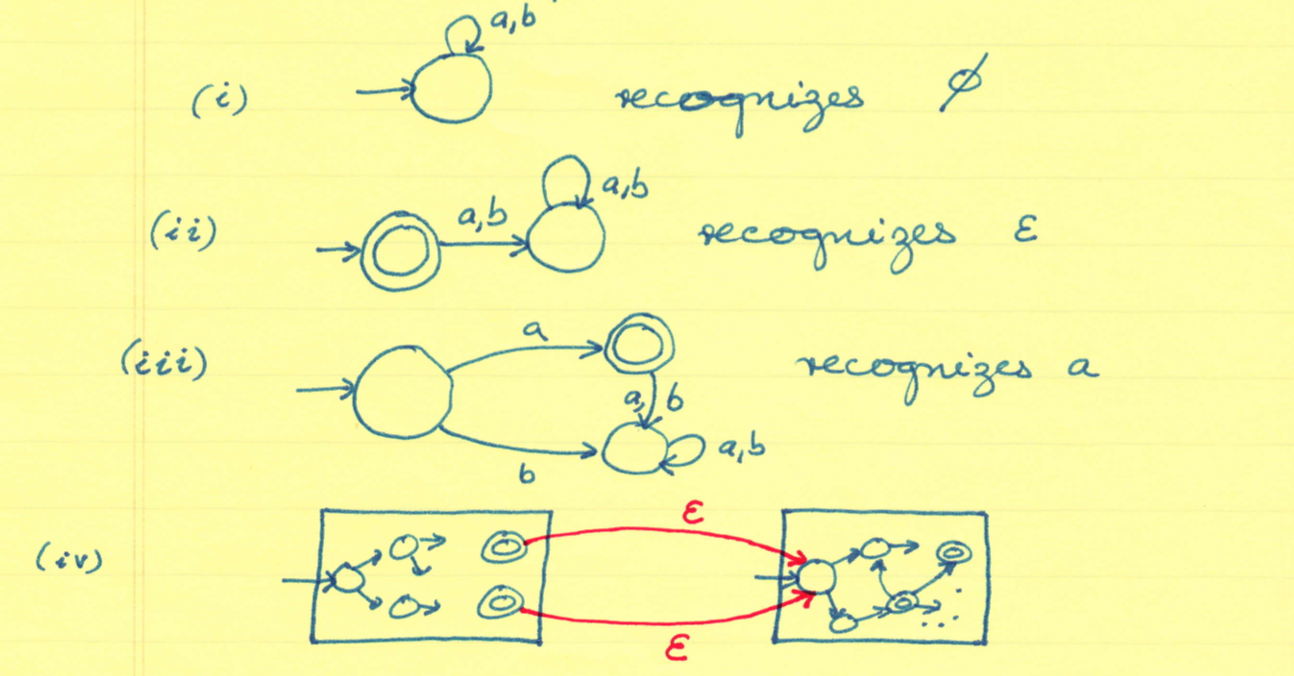
\includegraphics[scale = 0.7]{1.png}\\
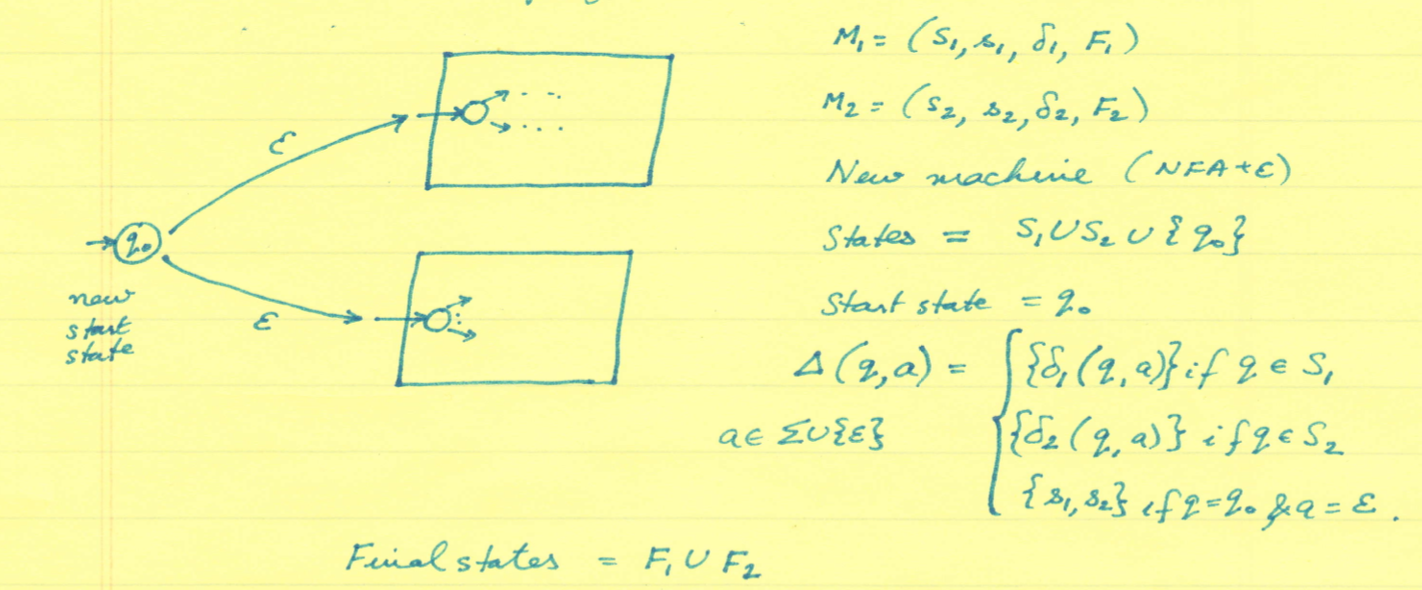
\includegraphics[scale = 0.7]{2.png}\\
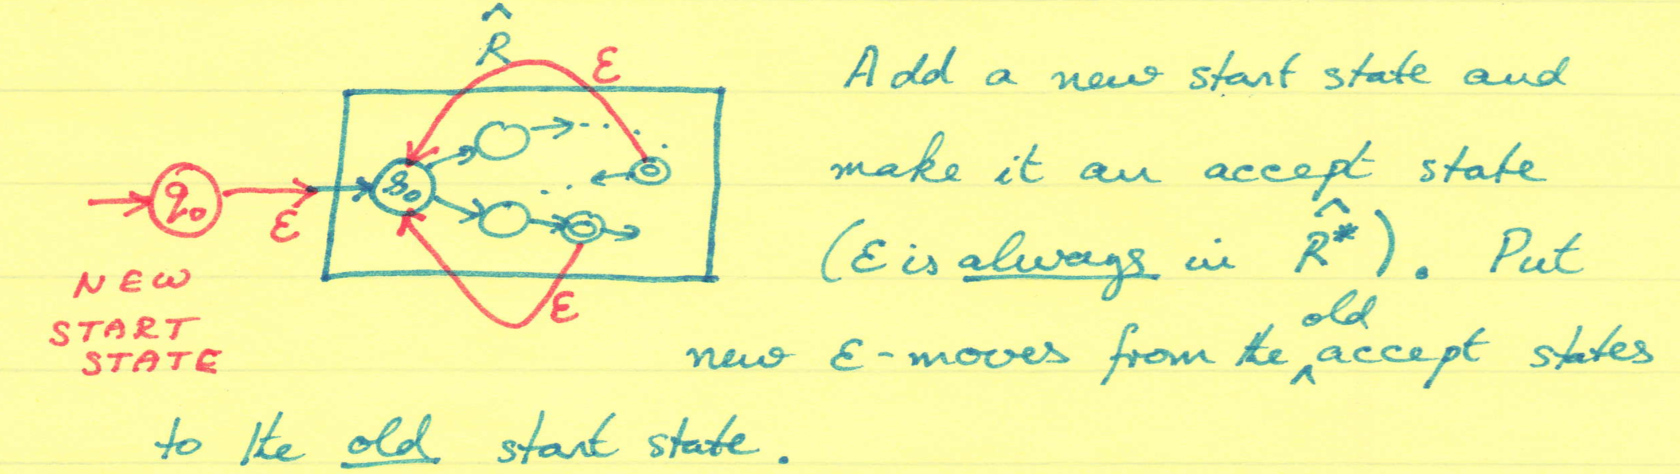
\includegraphics[scale = 0.55]{3.png}\\
\textbf{NOTE:} $q_0$ is the new start state as well as the accept state. It can accept word $\varepsilon$, and the next $\varepsilon$ is the $\varepsilon$ move.
\newpage
\section*{Example:}
$$L_1 = ab^*a \quad \quad  L_2 = (ba)^*\quad \quad  L_1\cdot L_2$$
\begin{center}
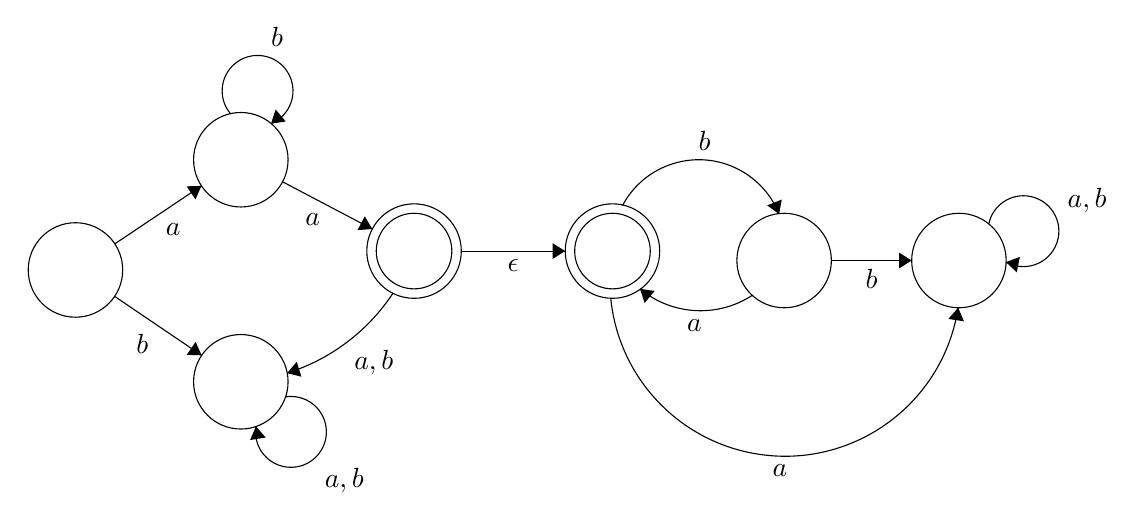
\begin{tikzpicture}[scale=0.2]
\tikzstyle{every node}+=[inner sep=0pt]
\draw [black] (11.1,-20.2) circle (3);
\draw [black] (21.6,-13.2) circle (3);
\draw [black] (32.6,-19) circle (3);
\draw [black] (32.6,-19) circle (2.4);
\draw [black] (21.6,-27.3) circle (3);
\draw [black] (45.2,-19) circle (3);
\draw [black] (45.2,-19) circle (2.4);
\draw [black] (56.1,-19.6) circle (3);
\draw [black] (67.2,-19.6) circle (3);
\draw [black] (13.6,-18.54) -- (19.1,-14.86);
\fill [black] (19.1,-14.86) -- (18.16,-14.89) -- (18.72,-15.72);
\draw (17.3,-17.2) node [below] {$a$};
\draw [black] (20.949,-10.283) arc (220.31354:-67.68646:2.25);
\draw (23.9,-6.07) node [above] {$b$};
\fill [black] (23.52,-10.91) -- (24.45,-10.77) -- (23.81,-10.01);
\draw [black] (13.59,-21.88) -- (19.11,-25.62);
\fill [black] (19.11,-25.62) -- (18.73,-24.76) -- (18.17,-25.59);
\draw (15.35,-24.25) node [below] {$b$};
\draw [black] (24.43,-28.26) arc (99:-189:2.25);
\draw (26.9,-33.55) node [right] {$a,b$};
\fill [black] (22.56,-30.13) -- (22.19,-31) -- (23.18,-30.84);
\draw [black] (24.25,-14.6) -- (29.95,-17.6);
\fill [black] (29.95,-17.6) -- (29.47,-16.79) -- (29.01,-17.67);
\draw (26.16,-16.6) node [below] {$a$};
\draw [black] (31.261,-21.676) arc (-33.41728:-72.5103:12.58);
\fill [black] (24.54,-26.75) -- (25.45,-26.98) -- (25.15,-26.03);
\draw (30.04,-25.29) node [below] {$a,b$};
\draw [black] (35.6,-19) -- (42.2,-19);
\fill [black] (42.2,-19) -- (41.4,-18.5) -- (41.4,-19.5);
\draw (38.9,-19.5) node [below] {$\epsilon$};
\draw [black] (45.837,-16.107) arc (-208.07137:-338.23006:5.492);
\fill [black] (55.78,-16.65) -- (55.95,-15.73) -- (55.02,-16.1);
\draw (51.05,-12.66) node [above] {$b$};
\draw [black] (54.101,-21.795) arc (-56.60978:-129.69166:6.017);
\fill [black] (46.95,-21.4) -- (47.24,-22.3) -- (47.88,-21.53);
\draw (50.4,-23.33) node [below] {$a$};
\draw [black] (59.1,-19.6) -- (64.2,-19.6);
\fill [black] (64.2,-19.6) -- (63.4,-19.1) -- (63.4,-20.1);
\draw (61.65,-20.1) node [below] {$b$};
\draw [black] (69.092,-17.287) arc (168.44395:-119.55605:2.25);
\draw (74.07,-15.79) node [right] {$a,b$};
\fill [black] (70.19,-19.7) -- (70.87,-20.35) -- (71.07,-19.37);
\draw [black] (67.149,-22.59) arc (-8.70252:-174.42193:11.121);
\fill [black] (67.15,-22.59) -- (66.53,-23.31) -- (67.52,-23.46);
\draw (55.84,-32.55) node [below] {$a$};
\end{tikzpicture}
\end{center}


\section*{From DFA to Regular expression:}
\begin{itemize}
	\item Let $Q = \{q_1,q_2, \ldots,q_n\}$ be the set of all automatons states
	\item Suppose $R^{(k)}_{ij}$ represents the set of all strings that transition the automaton from $q_i$ to $q_j$ without passing through any state higher than $q_k$
	\item We can construct the language $R_{ij}$ by successively constructing $R^{1}_{ij},R^2_{ij}, \ldots ,R^{n}_{ij} =R_{ij}$
	\item $R^{k}_{ij}$ is recursively defined as:
	 $$ R^k_{ij} = R^{k-1}_{ij} + R^{k-1}_{ik}(R^{k - 1}_{kk})^{*}R^{k-1}_{kj}$$
	 \item Assuming we have initialized $R^0_{ij}$ to be
	 $$R^0_{ij} =  \begin{cases}
	 	r \quad \text{ if } i \neq j \text{ and r transitions NFA from $q_i$ to $q_j$} \\
	 	r + \varepsilon\quad  \text{ if } i = j \text{ and r transitions NFA from $q_i$ to $q_j$}
	 	\\
	 	\emptyset \quad o.w.
	 \end{cases}$$
	 \item We always start in the order of $R^{0}_{ij}, R^{1}_{ij},R^2_{ij}, \ldots ,R^{n}_{ij}$
\end{itemize}



\section*{Equation between regular expression:}
\begin{itemize}
	\item $R\cdot (S+T) = R\cdot S + R\cdot T \quad \quad R + (S + T) = (R + S) + T \quad \quad  R + R = R$
	\item $R + \emptyset = R \quad \quad R + S = S + R \quad \quad R \cdot \varepsilon = R$
	\item $\varepsilon \cdot R = R \cdot \varepsilon \quad \quad R\cdot (S \cdot T) = (R\cdot S) \cdot T $
	\item $\varepsilon + R^* R = \varepsilon + R R^* = R^*$
\end{itemize}

\newpage
\textbf{DATE: 9-19 LECTURE 7}
\section*{Minimization of DFA}
To begin with, we define an equivalence relation on state\\
Use equivalence classes to define a new smaller machine.\\
\newline
\textbf{Definition:} Given a DFA, $M =\{  S, S_0, \delta, F \} $ over $\Sigma$, we say $P \approx S$, if 
$$ \forall x \in \Sigma^*, \delta^*(p, x) \in F \Leftrightarrow \delta^*(q, x) \in F $$\\
\newline
\textbf{REMARK:} NOT equivalent?\\
$$ \exists x \in \Sigma^* \begin{cases}
	\delta^*(p, x) \in F \text{ while } \delta^*(q, x) \notin F\\
		\delta^*(p, x) \notin F \text{ while } \delta^*(q, x) \in F
\end{cases} $$
\\
\newline
\textbf{Lemma A:} $p \approx q \implies \forall a \in \Sigma, \delta(p, a)  \approx\delta(q, a)   $
\begin{proof}
	Suppose that $\delta^*(\delta( p, a ), x )\in F $, then we can say that $ \delta^*(p, ax ) \in F $ \\
	As we know that $p \approx q$, according to the definition we can say $ \delta^*(p, ax) \in F \Leftrightarrow \delta^*(q, ax) \in F  $\\
	So, we can say that $ \delta^*(\delta( q, a ), x )\in F  $\\
	Thus, we can say $\delta(p, a)  \approx \delta(q, a) $\\
\end{proof}
\textbf{Lemma A*:}
$\forall  x \in \Sigma^*, \delta^* ([p],x)=[\delta^*(p, x)]$\\
We can prove this via induction on the length of the string\\
\newline


\textbf{REMARK:} $p \approx q$ can be written as $[p] = [q]$, so the lamma can be written as $[p] = [q] \implies [\delta(p, a)]  = [\delta(q, a)] $ 
\section*{quotient machine}
Next, we define the concept of a \textbf{quotient machine}: $M/\approx =(S',s'_0, \delta',F')$
 (with the same alphabet $\Sigma$ ), where:
 \begin{itemize}
 	\item $S' = \{[s]\quad | s \in S\}\quad \quad (s/ \approx)$ (the set of all equivalence classes)
	\item $s'_0=[s_0]$
	\item $F' =\{[p]| p\in F \}$ (the set of equivalence classes for accept states)
	\item $\delta' : Q'\times \Sigma \to Q'$ is defined by  $ \delta'([p], a) = [\delta(p, a)]  $
 \end{itemize}
 \textbf{Lemma B}: $p \in F, p \approx q \implies q \in F$\\
 Using definition and $\varepsilon$ to prove this.\\
 \newline
 \textbf{Lemma C}: $\forall w \in \Sigma^*, \delta'^*([p], w) = [ \delta^*(p, w) ] $
\begin{proof}
	Prove by induction:
	\begin{itemize}
		\item Base Case: $w = \varepsilon$, then we have $ \delta'^*([p], \varepsilon ) = [p] =  [ \delta^*(p, \varepsilon ) ] $
		\item Inductive Step: Suppose that $\delta'^*([p], w) = [ \delta^*(p, w) ]$, then we need to prove that: $\delta'^*([p], wa) = [ \delta^*(p, wa) ]$
		\begin{align*}
			\delta'^*([p], wa) 
			&= \delta'\bigg(\delta'^*([p], w), a \bigg)\\
			&= \delta'\bigg([ \delta^*(p, w) ], a \bigg) \textbf{ according to hypothesis} \\
			&= \bigg[\delta( \delta^*(p, w)  ,a  )  \bigg] \textbf{ according to the definition of } \delta' \\
			&= [\delta(p, wa) ]
		\end{align*}
	\end{itemize}
\end{proof}
\textbf{Theorem:} $L(M') = L(M) $
\begin{proof}
	\begin{align*}
		x \in L(M') 
		&\Leftrightarrow \delta'^*([s_0], x) \in F'\\
		&\Leftrightarrow [\delta^*(s_0, x)] \in F'\\
		&\Leftrightarrow \delta^*(s_0, x) \in F\\
		&\Leftrightarrow x \in L(M)
	\end{align*}
\end{proof}
\section*{Distinguishable:}
$ p\quad \Bowtie \quad q := \exists w \in \Sigma $ such that $\begin{cases}
	\delta*(p, w) \in F \quad \delta*(q, w) \notin F \\
	(or) \quad  \delta*(p, w) \notin F \quad \delta*(q, w) \in F\\
\end{cases}$
\\Fact: if $\exists a \in \Sigma, $ such that $\delta(p, a)\quad \Bowtie \quad \delta(q, a)$, then $ p\quad \Bowtie \quad q $
\section*{Algorithm:}
Define a $S \times S$ array of booleans:
\begin{itemize}
	\item[1]: for every pair (p, q) such that $p \in F $ and $q \notin F$, we put a 0 at position $(p, q)$ of the matrix
	\item[2]: Repeat until no more change:\\
	For each pair of $(p, q)$ not marked 0, check if $\exists a \in \Sigma$, such that $(\delta(p, a),\delta(q, a) ) $ is 0. If yes, then mark $(p, q)$ as 0
	\item[3]: mark everything else as 1\\
\end{itemize}

\newpage
\begin{center}
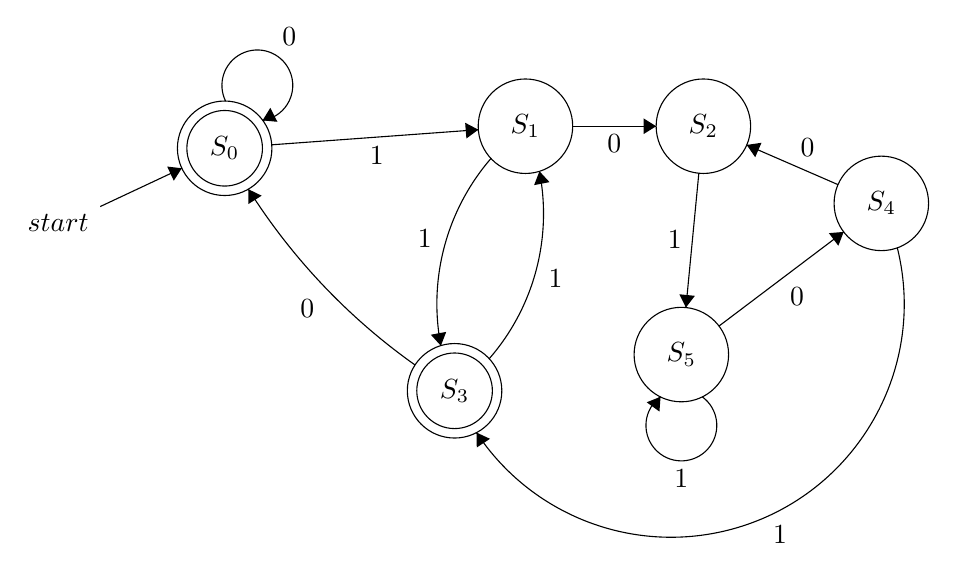
\begin{tikzpicture}[scale=0.2]
\tikzstyle{every node}+=[inner sep=0pt]
\draw [black] (14.4,-20.5) circle (3);
\draw (14.4,-20.5) node {$S_0$};
\draw [black] (14.4,-20.5) circle (2.4);
\draw [black] (33.5,-19.1) circle (3);
\draw (33.5,-19.1) node {$S_1$};
\draw [black] (44.8,-19.1) circle (3);
\draw (44.8,-19.1) node {$S_2$};
\draw [black] (56.1,-24) circle (3);
\draw (56.1,-24) node {$S_4$};
\draw [black] (29,-35.9) circle (3);
\draw (29,-35.9) node {$S_3$};
\draw [black] (29,-35.9) circle (2.4);
\draw [black] (43.4,-33.6) circle (3);
\draw (43.4,-33.6) node {$S_5$};
\draw [black] (14.463,-17.512) arc (206.52557:-81.47443:2.25);
\draw (18.51,-14.01) node [above] {$0$};
\fill [black] (16.81,-18.73) -- (17.75,-18.82) -- (17.3,-17.93);
\draw [black] (17.39,-20.28) -- (30.51,-19.32);
\fill [black] (30.51,-19.32) -- (29.67,-18.88) -- (29.75,-19.88);
\draw (24.06,-20.37) node [below] {$1$};
\draw [black] (28.128,-33.035) arc (-169.15161:-220.83855:14.119);
\fill [black] (28.13,-33.04) -- (28.47,-32.16) -- (27.49,-32.34);
\draw (27.59,-26.21) node [left] {$1$};
\draw [black] (34.386,-21.96) arc (11.0887:-41.07885:14.016);
\fill [black] (34.39,-21.96) -- (34.05,-22.84) -- (35.03,-22.65);
\draw (34.94,-28.79) node [right] {$1$};
\draw [black] (26.488,-34.26) arc (-125.3097:-147.74535:39.543);
\fill [black] (15.9,-23.1) -- (15.91,-24.04) -- (16.75,-23.51);
\draw (20.12,-30.67) node [left] {$0$};
\draw [black] (36.5,-19.1) -- (41.8,-19.1);
\fill [black] (41.8,-19.1) -- (41,-18.6) -- (41,-19.6);
\draw (39.15,-19.6) node [below] {$0$};
\draw [black] (53.35,-22.81) -- (47.55,-20.29);
\fill [black] (47.55,-20.29) -- (48.09,-21.07) -- (48.49,-20.15);
\draw (51.42,-21.04) node [above] {$0$};
\draw [black] (44.51,-22.09) -- (43.69,-30.61);
\fill [black] (43.69,-30.61) -- (44.26,-29.87) -- (43.27,-29.77);
\draw (43.46,-26.27) node [left] {$1$};
\draw [black] (45.79,-31.79) -- (53.71,-25.81);
\fill [black] (53.71,-25.81) -- (52.77,-25.89) -- (53.37,-26.69);
\draw (50.75,-29.3) node [below] {$0$};
\draw [black] (57.113,-26.818) arc (13.97449:-146.56055:14.807);
\fill [black] (30.39,-38.55) -- (30.41,-39.5) -- (31.25,-38.95);
\draw (49.67,-44.46) node [below] {$1$};
\draw [black] (6.5,-24.2) -- (11.68,-21.77);
\draw (5.79,-25.24) node [left] {$start$};
\fill [black] (11.68,-21.77) -- (10.75,-21.66) -- (11.17,-22.56);
\draw [black] (44.723,-36.28) arc (54:-234:2.25);
\draw (43.4,-40.85) node [below] {$1$};
\fill [black] (42.08,-36.28) -- (41.2,-36.63) -- (42.01,-37.22);
\end{tikzpicture}
\end{center}
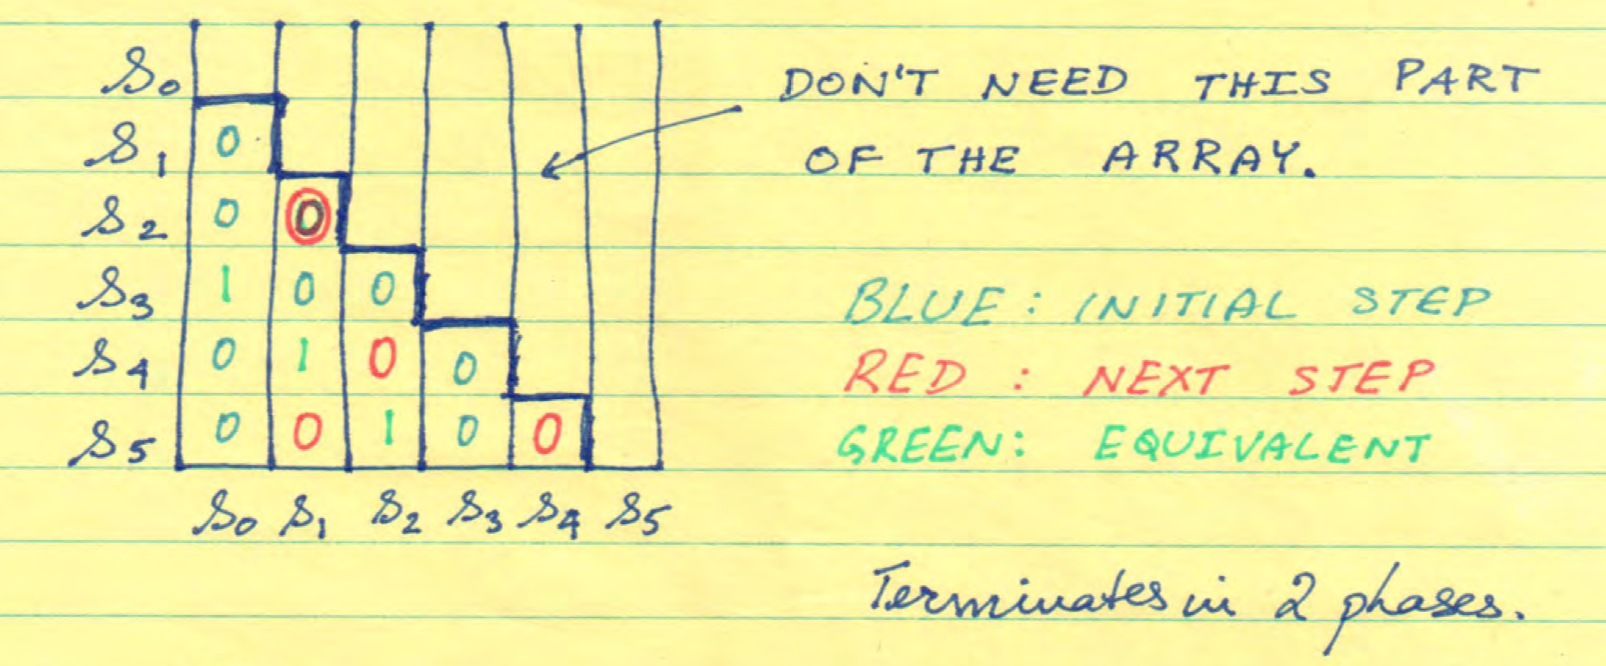
\includegraphics[scale = 0.6]{4.png}
The first step we will make (0,1), (0,2), (0,4), (0,5), (1,3), (2,3), (3,4), (3,5) be 0\\
\newline
The second step we will make (1,2), (1,5), (2,4), (4,5) be 0\\

 

\end{document}